\chapter{Principal Components Analysis \label{chapter:pca}}

Clustering (Chapter~\ref{chapter:clustering}) is one approach to uncovering latent structure in data. Another are matrix decomposition methods, the most famous of which is \textbf{principal components analysis (PCA)}. PCA is a powerful statistical tool for analyzing and visualizing datasets. It has been independently discovered several times over the course of history, and can be formulated mathematically a few different ways.

%%%%%%%%%%%%%%%%%%%%%%%%%%%%%%%%%%%%%%%%%%%%%%%%%%%%%%%%%%%%%%%%%%%%%%%%%%%%%

\section{Principal Components: What are they?}

You can think of PCA as a rotation of the feature space onto a set of axes that most efficiently represent the data. The \textbf{principal components} are these axes, or \textbf{basis vectors}. Here are pictures of the first two principal components for a small dataset. These were borrowed from Andrew Ng's lecture notes for CS229 at Stanford University. 

\begin{center}
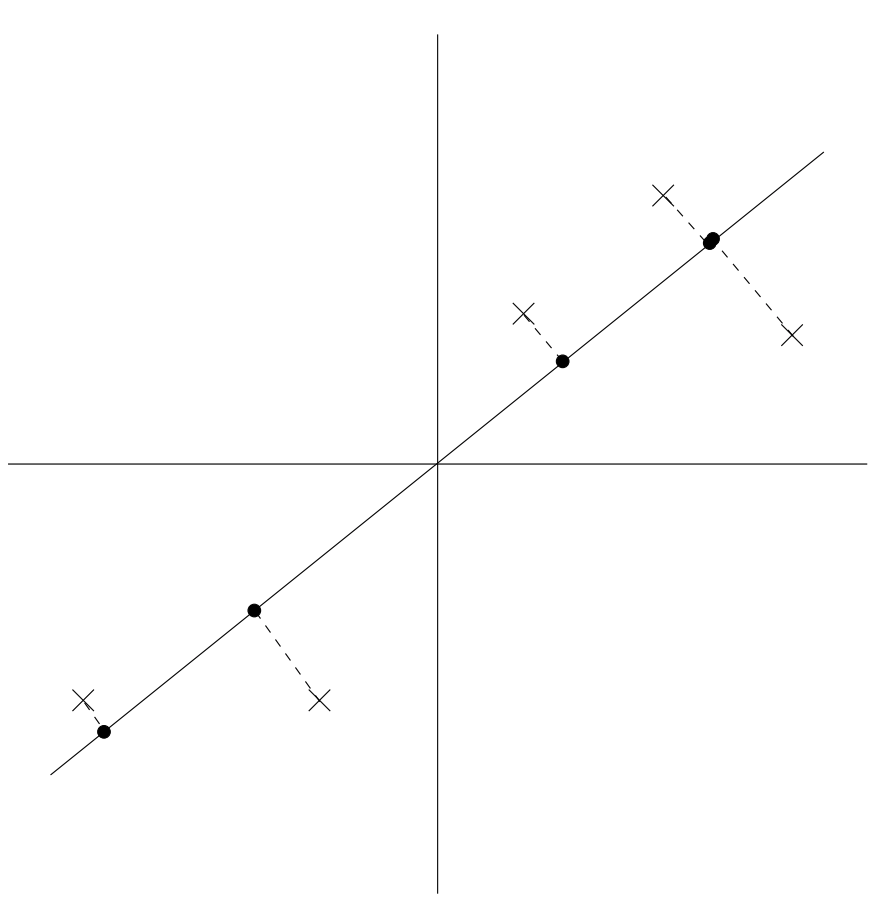
\includegraphics[width=0.7\textwidth]{img/l04-ang-pc1.png}
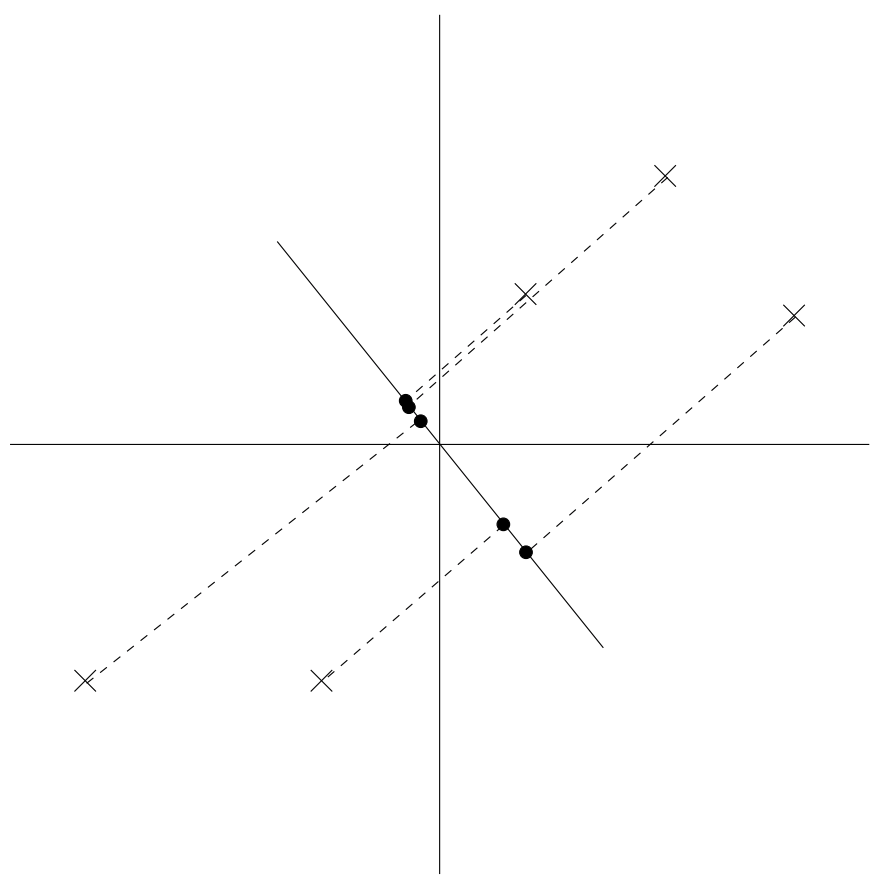
\includegraphics[width=0.7\textwidth]{img/l04-ang-pc2.png}
\end{center}

\begin{question}{}
What do you notice about principal components 1 (top) and 2 (bottom)? Think in terms of (a) the variance (spread) of the data, and (b) the projection errors (dotted lines). 
\end{question}

Mathematically, PCA is a linear projection of $p$-dimensional datapoints, $x^{(1)}, \dots, x^{(n)}$ onto a $k$-dimensional space ($k \leq p$) defined by basis vectors $u_1, \dots, u_k$ such that:
\begin{itemize}
\item the projection maximizes the variance from the original dataset that is retained
\item the projection minimizes projection error (square loss)
\item the basis vectors, $\left\{u_1, \dots, u_k\right\}$, are orthogonal (i.e., perpendicular)
\end{itemize}

The number of distinct principal components is the smaller of the number of original variables ($p$) or the number of observations ($n$) minus one.

%%%%%%%%%%%%%%%%%%%%%%%%%%%%%%%%%%%%%%%%%%%%%%%%%%%%%%%%%%%%%%%%%%%%%%%%%%%%%

\section{Definitions}

\subsection{Feature Vectors}

Say you have $n$ samples in a dataset, and each has dimensionality $p$. Let $x^{(i)}$ be the vector of $p$ features for the $i$th person. We write

$$ x^{(i)} = \begin{bmatrix}
           x_{1}^{(i)} \\
           x_{2}^{(i)} \\
           \vdots \\
           x_{p}^{(i)}
         \end{bmatrix} $$
        
\noindent and we can write our entire dataset as a $n \times p$ matrix like this:

$$ X = \begin{bmatrix}
x_1^{(1)} & x_2^{(1)} & \dots & x_p^{(1)} \\
x_1^{(2)} & x_2^{(2)} & \dots & x_p^{(2)} \\
\vdots & \vdots & \ddots & \vdots \\
x_1^{(n)} & x_2^{(n)} & \dots & x_p^{(n)} \\
\end{bmatrix} $$ 
such that the $i$th row of the matrix is the vector of features for the $i$th person. This is exactly the same notation that we have used in previous chapters.  

\subsection{Variance and Covariance \label{ssect:varcovar}}

The \textbf{sample covariance} of two features $x_j$ and $x_k$ is given by
$$ \text{cov}(x_j, x_k) = S_{jk} = \frac{1}{n-1} \sum_{i=1}^{n}\left(x_j^{(i)}-\overline{x_j}\right) \left(x_k^{(i)}-\overline{x_k}\right) $$
where the bar ($\overline{x_j}$) refers to the mean of $x_j$ across the entire dataset. We can also write it in matrix format as
$$ S = \frac{1}{n-1} \sum_{i=1}^n (x^{(i)} - \overline{x})(x^{(i)} - \overline{x})^T. $$

The covariance can be any real number between positive and negative infinity. One weird thing about it is that it has units - the product of the units of the two features. This means that the covariance depends on the scale that is chosen for each feature, which is somewhat arbitrary. The \textbf{sample variance} of a given feature is just the covariance in cases where $j = k$ (the covariance of a feature with itself). 

The \textbf{correlation} (technically the \textbf{Pearson correlation}) is a unitless, normalized version of the covariance and has the form
$$ \text{cor}(x_j, x_k)=\frac{\sum_{i=1}^{n}(x_j^{(i)}-\overline{x_j})(x_k^{(i)}-\overline{x_k})}{\sqrt{\sum_{i=1}^{n}(x_j^{(i)}-\overline{x_j})^2}{\sqrt{\sum_{i=1}^{n}(x_k^{(i)}-\overline{x_k})^2}}}. $$

\subsection{Orthogonality}

Two vectors are \textbf{orthogonal} if their \textbf{inner product}, or \textbf{dot product}, is zero. This is defined as
$$ \langle x, y \rangle = x \cdot y = \sum_{i=1}^n x_i y_i $$
where the sum is over the vector components. If this mathematical notation makes you uncomfortable, just think of ``orthogonality'' as ``perpendicularity'' and you'll be able to understand it visually. 

In PCA, the vectors whose inner products we are concerned with will \emph{not} be the feature vectors for individual samples. They will be, instead, the \emph{columns} of $X$ -- the values of a single feature for all $n$ samples. 

%%%%%%%%%%%%%%%%%%%%%%%%%%%%%%%%%%%%%%%%%%%%%%%%%%%%%%%%%%%%%%%%%%%%%%%%%%%%%%%%%%%%%%%%%%%%

\section{Example: Running PCA in R}

Let's say you have measurements of weight, height, and IQ ($p=3$) for $n=100$ men. Here are the first $10$ rows of the $100$ row dataset:

\begin{center}
\begin{tabular}{cccc}
Patient ID ($i$) & Height (in) & Weight (lbs) & IQ \\
\midrule
1 & 74.9 & 155.6 & 109 \\
2 & 66.5 & 171.6 & 117 \\
3 & 74.4 & 175.2 & 91 \\
4 & 65.8 & 151.3 & 84 \\
5 & 70.2 & 162.7 & 107 \\
6 & 78.8 & 206.4 & 117 \\
7 & 69.1 & 162.7 & 96 \\
8 & 70.6 & 150.3 & 110 \\
9 & 65.2 & 156.2 & 121 \\
10 & 66.8 & 153.3 & 93 \\
\end{tabular}
\end{center}

\noindent Here are some scatterplots showing pairwise comparisons of the three features:

\begin{center}
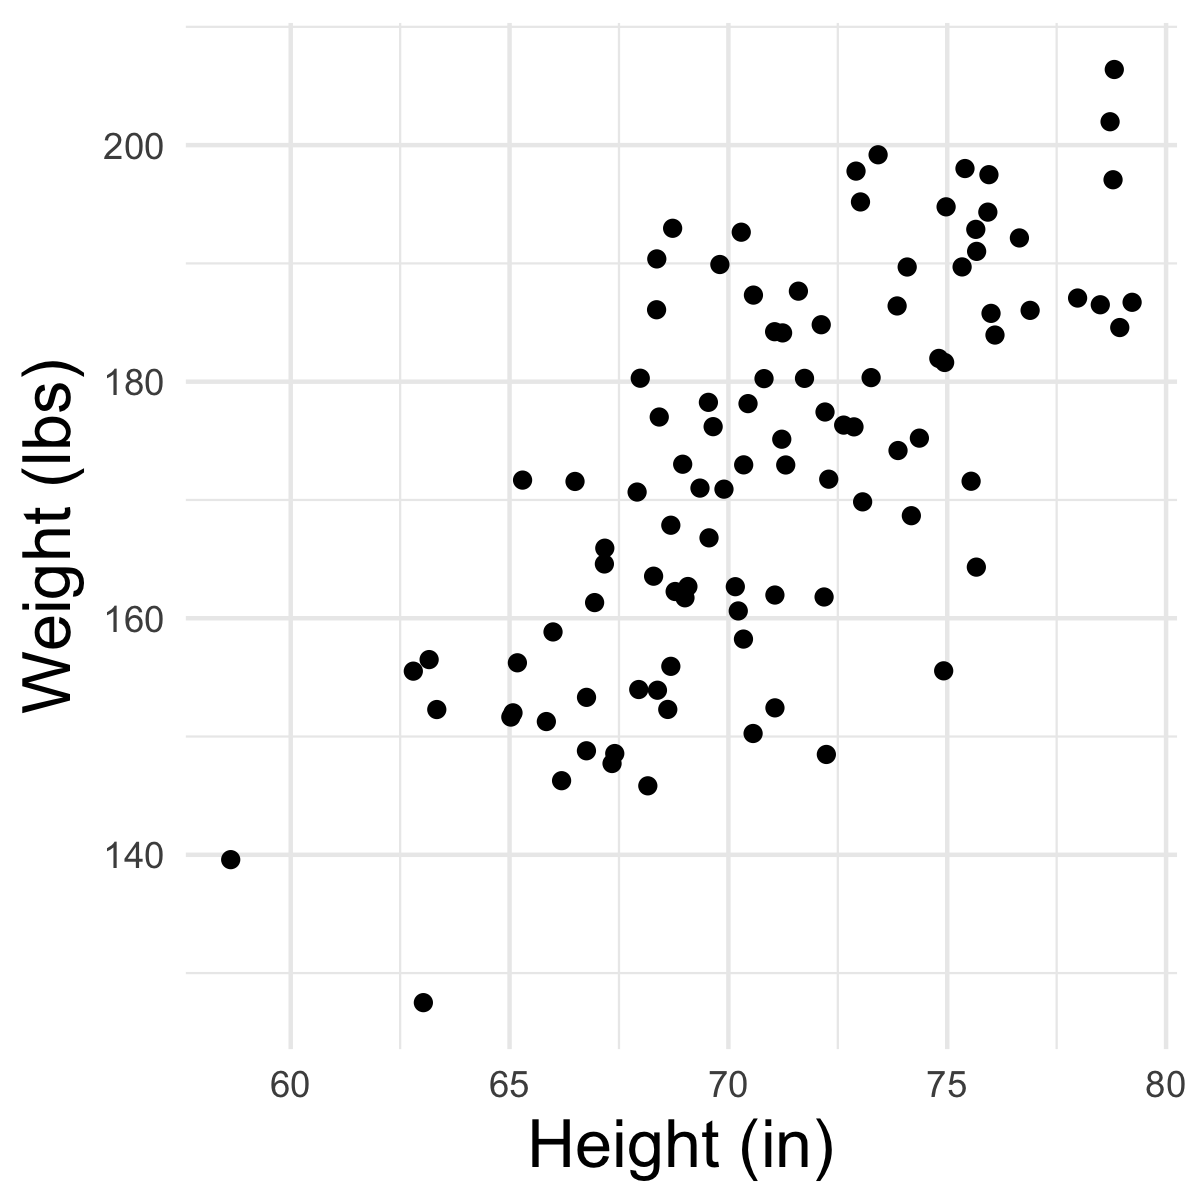
\includegraphics[width=0.32\textwidth]{img/l04-example-1.png}
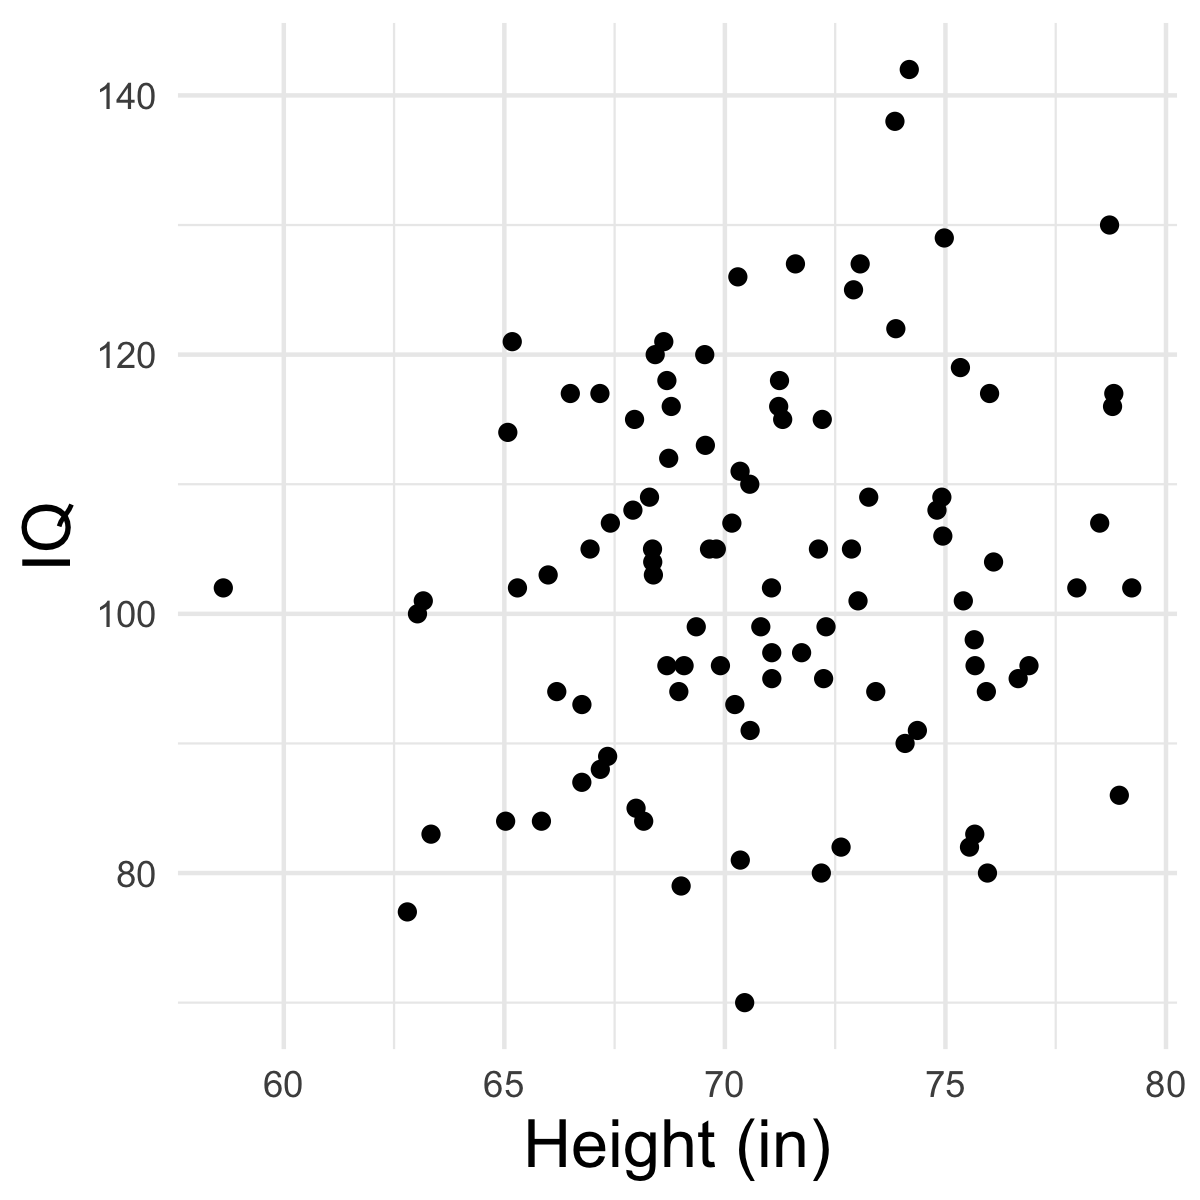
\includegraphics[width=0.32\textwidth]{img/l04-example-2.png}
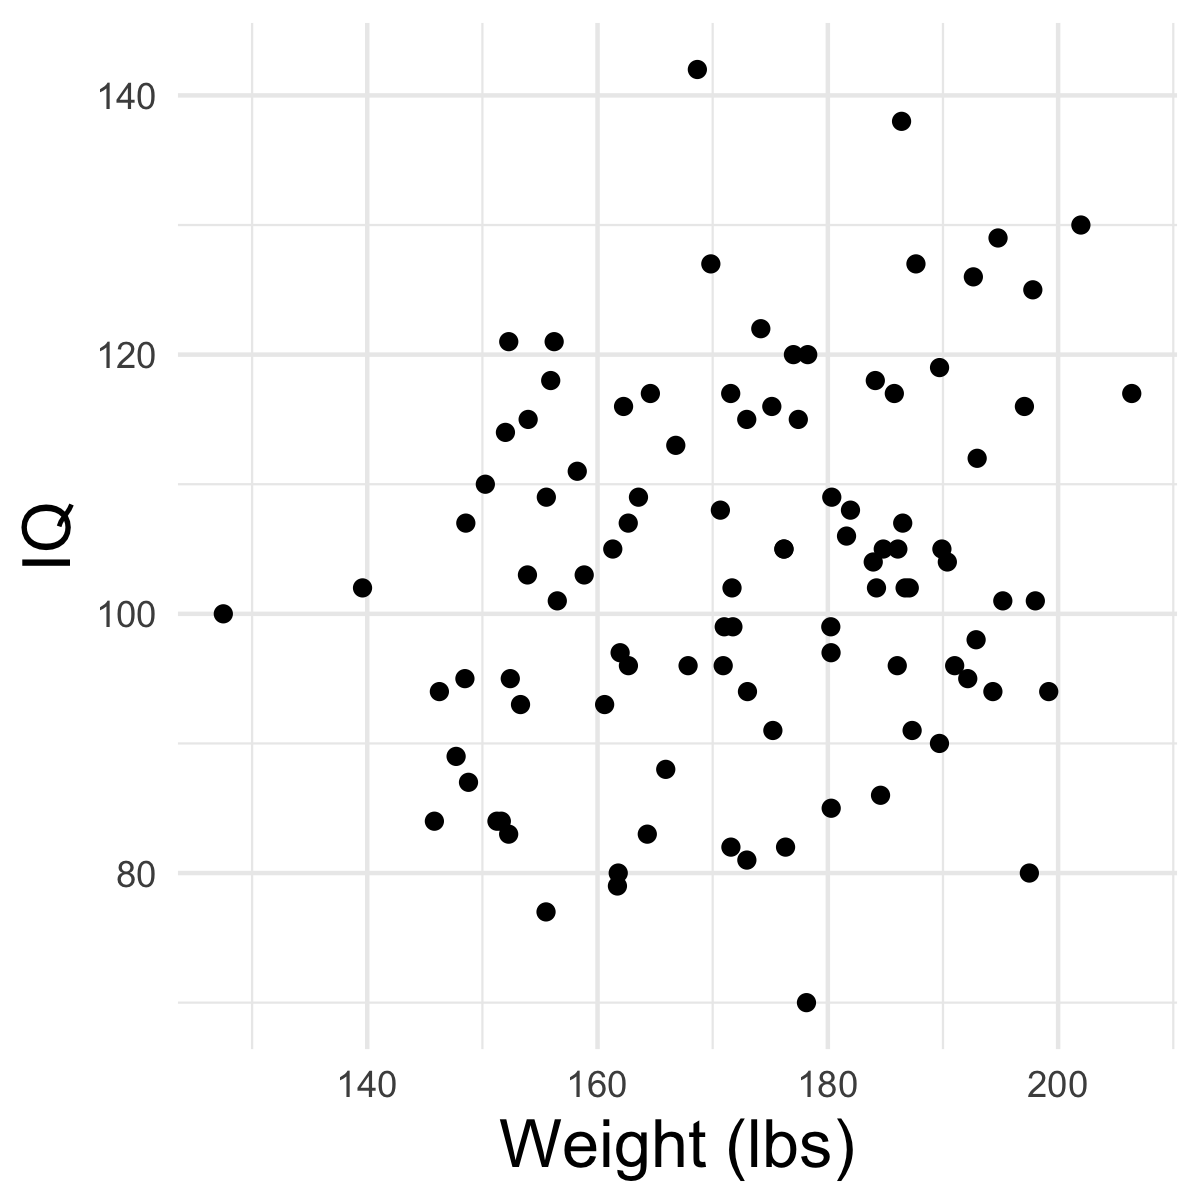
\includegraphics[width=0.32\textwidth]{img/l04-example-3.png}
\end{center}

\noindent The \textbf{correlation matrix} for these data looks like this:

\begin{verbatim}
       height weight     iq
height  1.000  0.790 -0.103
weight  0.790  1.000 -0.078
iq     -0.103 -0.078  1.000
\end{verbatim}

\vspace{2mm}

\begin{question}{}
Looking at the correlation matrix, which features are most tightly correlated? What does this imply about the direction of the first principal component, PC1? 
\end{question}

\subsection{Centering and Scaling}

PCA is sensitive to the relative scales of the different variables in the original dataset. For this reason, datasets are usually \emph{scaled} and \emph{centered} before PCA is performed. All this means is that for each column (feature) of the dataset, we subtract its mean and divide by its standard deviation. The transformed column will have mean 0 and standard deviation 1. 

If the data are scaled and centered, we can rewrite $S$ (the sample covariance matrix from Section~\ref{ssect:varcovar}) as $X^T X/(n-1)$.

\vspace{2mm}

\begin{question}{}
What would happen to the principal components if you didn't center and scale the data?
\end{question}

\begin{question}{}
Why do you think the interpretation of the principal components becomes more difficult if you have features measured on lots of different scales (e.g., some categorical, some numeric/roughly normal, some numeric/highly skewed)? 
\end{question}

\subsection{Input and Output}

In R, we can run PCA on our dataset, \texttt{d}, using the following command:
\begin{center}
\verb|p <- prcomp(d[,2:4], center = TRUE, scale. = TRUE, rank. = 3)|
\end{center}
where \texttt{rank.} is an optional parameter indicating the number, $k$, of principal components desired. The output looks like this:

\begin{multicols}{2}
{\scriptsize
\begin{verbatim}
> p$sdev
[1] 1.3454074 0.9899765 0.4580672

> p$rotation
              PC1         PC2         PC3
height  0.6996236 -0.09446119 -0.70823998
weight  0.6971414 -0.12698944  0.70559726
iq     -0.1565906 -0.98739595 -0.02299201

> p$center
   height    weight        iq 
 70.74468 174.43346 101.12000 
 
> p$scale
   height    weight        iq 
 3.914989 13.853272 14.183701 
 
> p$x
                PC1          PC2          PC3
  [1,] -0.189268854  1.976180297 -0.416704298
  [2,]  1.794925031  0.710160037  0.575478783
  [3,] -0.404617344  0.283418147  0.151536071
  [4,] -0.471675025 -0.710146894  0.347006397
  [5,] -1.073877096 -0.234684815 -0.638243675
  [6,] -0.654663317  0.043481120 -0.107082277
  [7,] -1.705841441  0.368990046 -0.794047654
  [8,]  2.311353981 -0.501565781  0.033112309
  [9,] -0.006387264 -0.535422493 -1.126177513
 [10,] -1.557136911  1.399023167 -0.045281059
 [11,]  2.632974868 -1.046037442 -0.239934797
 [12,] -0.978337630 -0.193476727  0.007814938
 [13,] -0.625980903 -0.456274882 -0.305349616
 (continued)
\end{verbatim}
}
\end{multicols}

\begin{question}{}
Describe/draw the directions of the three principal component vectors, PC1, PC2, and PC3, in the coordinate system of the original predictors, height, weight, and IQ.
\end{question}

\begin{question}{}
Here is a picture of the flow cytometry dataset we first encountered in Chapter~\ref{chapter:clustering}.
\begin{center}
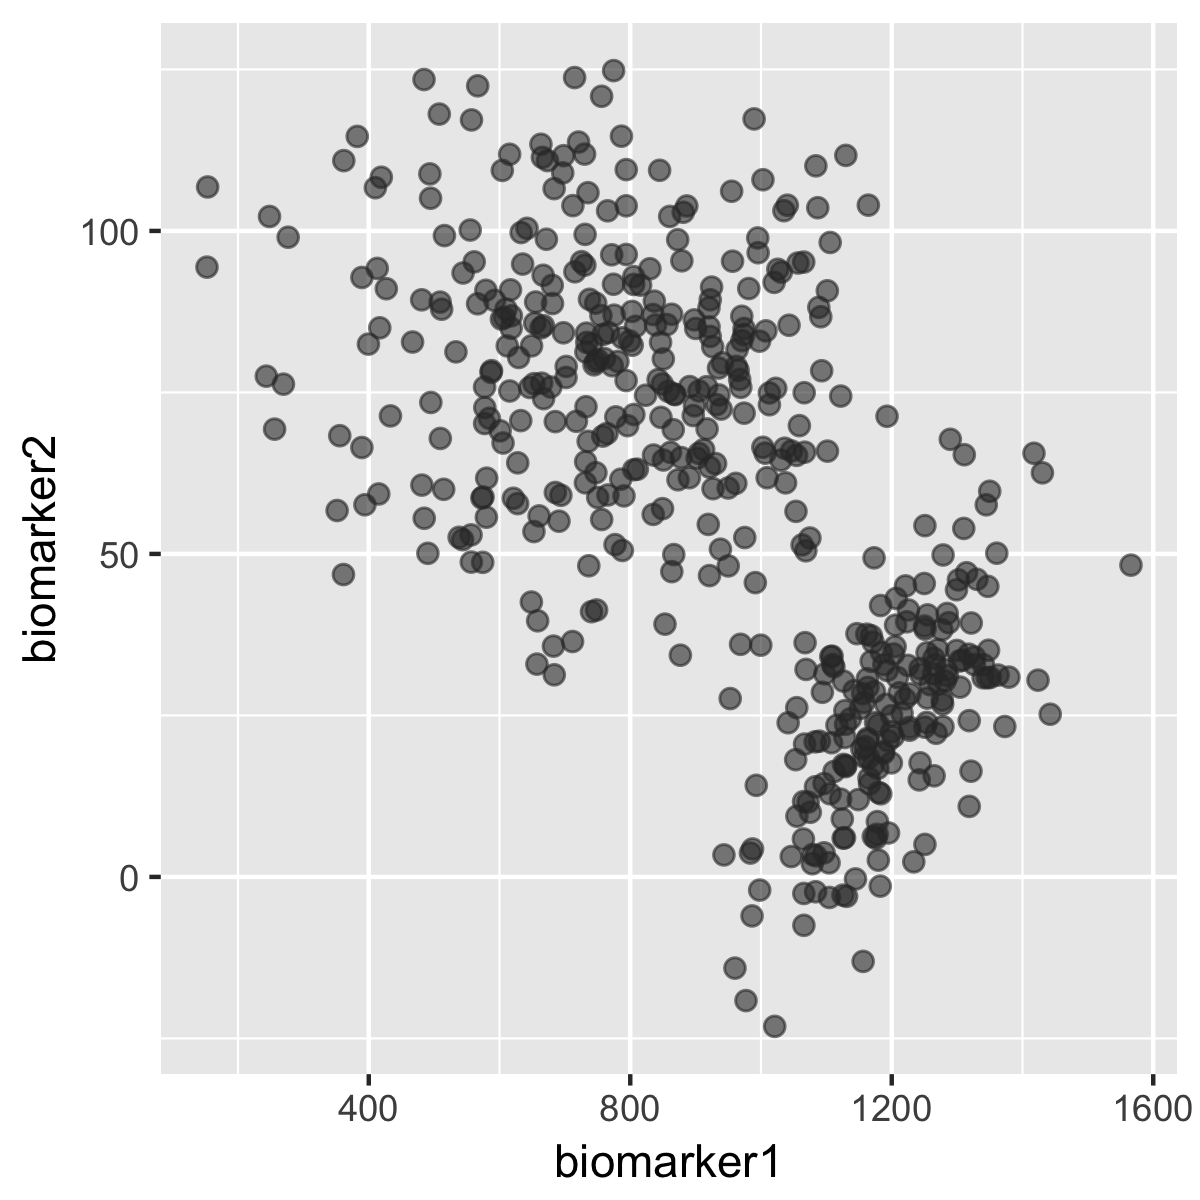
\includegraphics[width=0.7\textwidth]{img/biomarker-data-big-no-labels.png}
\end{center}
What would PC1 and PC2 look like for this dataset? (Why is there no PC3?) How could PCA help you separate the two clusters?
\end{question}

%%%%%%%%%%%%%%%%%%%%%%%%%%%%%%%%%%%%%%%%%%%%%%%%%%%%%%%%%%%%%%%%%%%%%%%%%%%%%%%%

\section{Applications of PCA}

\subsection{Eigenfaces}

Eigenfaces were an early application of PCA to computer vision, specifically image search and retrieval. Here's what you do to create a set of eigenfaces:
\begin{enumerate}
\item Prepare training set of images taken under the same lighting conditions, with mouths and eyes aligned, resampled to a common pixel resolution.
\item Generate a vector for each image by concatenating the pixel intensities across the rows. So if the image is of dimension $r \times c$, the image vector will have $p = rc$ features.
\item Create the data matrix from the $n$ vectors.
\item Center the data (Why wouldn't we scale the data?).
\item Calculate the eigenvectors and eigenvalues of the sample covariance matrix. Each eigenvector corresponds to one eigenface. 
\end{enumerate}

Some real eigenfaces are shown below \footnote{Figure details: (top) some of the original faces from the training set (there were 86 images total); (bottom) the eigenfaces corresponding to the 18 largest eigenvalues of the covariance matrix. From https://www.clear.rice.edu/elec301/Projects99/faces/images.html.}. 

\begin{center}
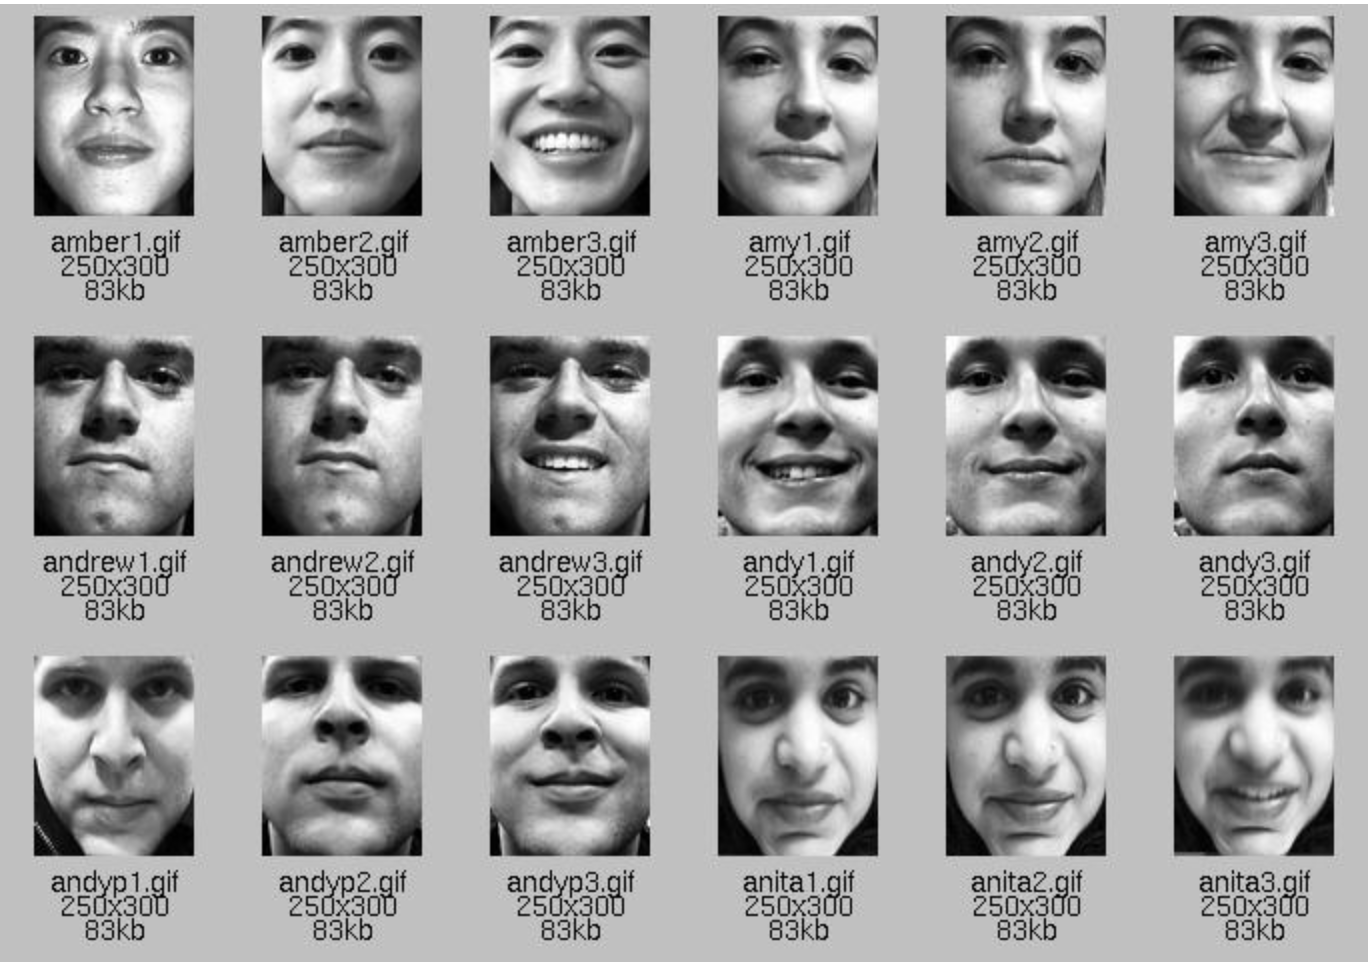
\includegraphics[width=0.8\textwidth]{img/l04-eigenfaces-1.png}\\[5mm]
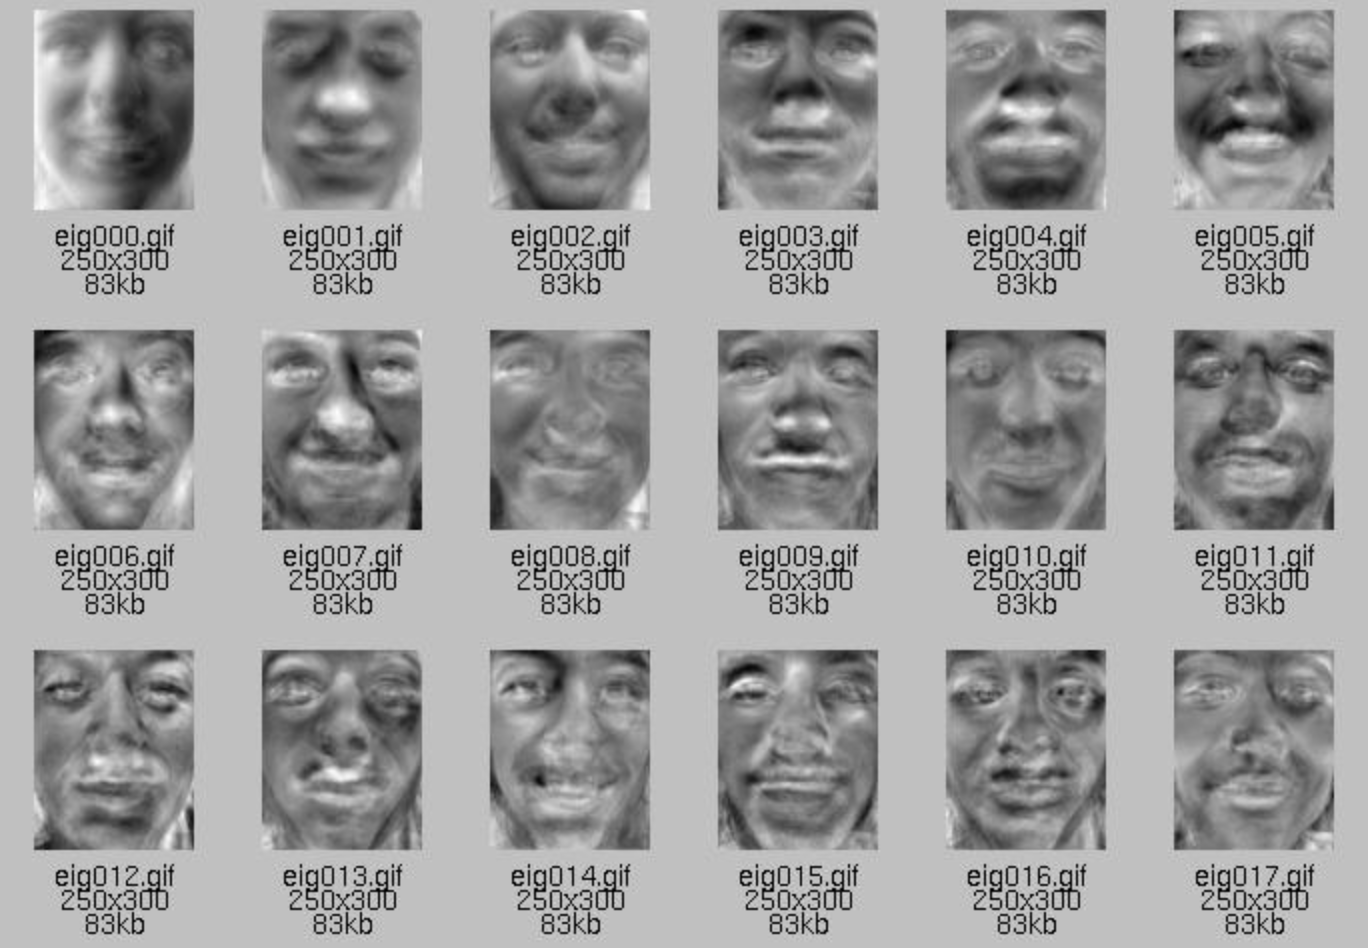
\includegraphics[width=0.8\textwidth]{img/l04-eigenfaces-2.png}
\end{center}

\begin{question}{}
What is $X$ for the eigenfaces problem? What are the principal components? How could you use the principal components to match a new face to an existing database of faces?
\end{question}

\subsection{Image Compression}

PCA can also be used for image compression. In that case, the raw pixels for the image are the data matrix, $X$ (so each ``sample'' is one row of the image and each ``feature'' is one column of the image). Generally the data are centered but not scaled here (Why?). A subset of the principal components corresponding to the $r$ largest eigenvalues are used to reconstruct the image. The picture below illustrates the process\footnote{Figure: Using PCA for image compression. The image is recomposed by adding together many gridlike images like that shown in (a). From \texttt{https://www.projectrhea.org/rhea/index.php/PCA\_Theory\_Examples}.}. 

\begin{center}
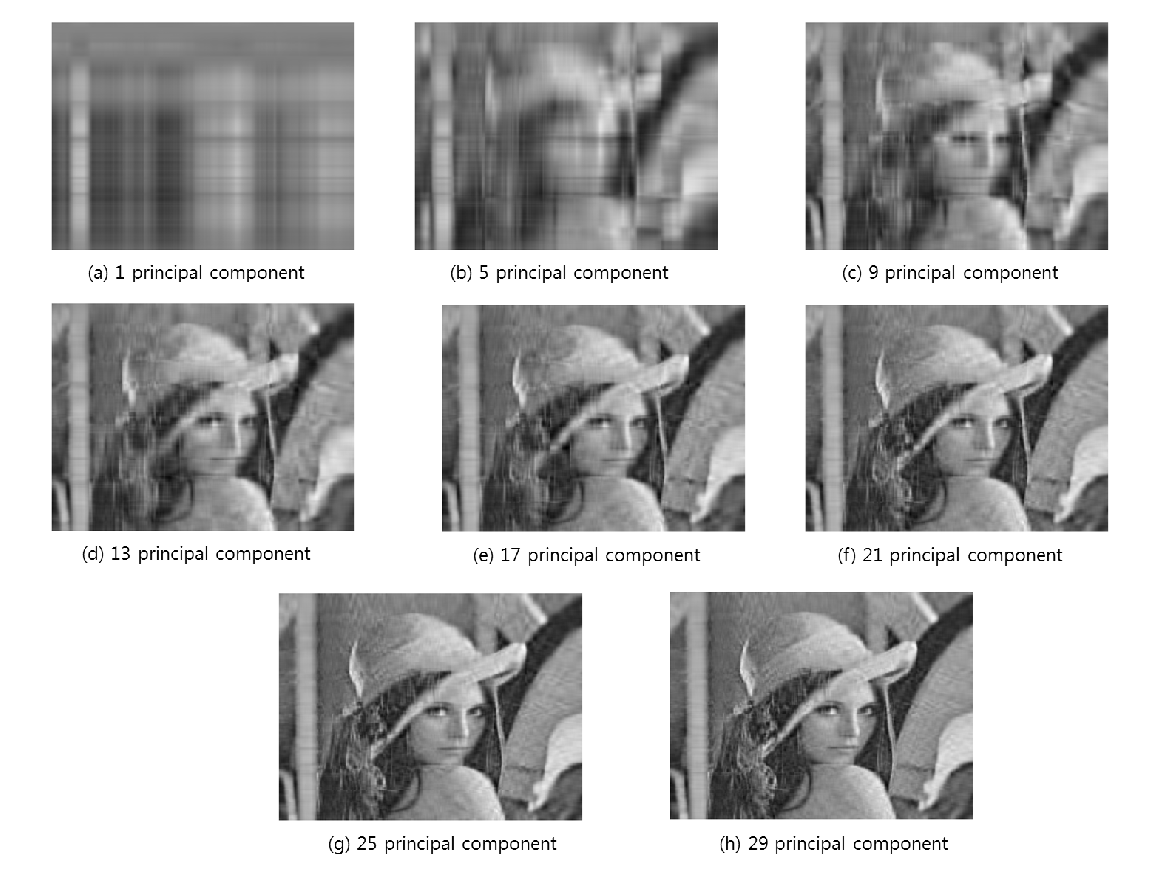
\includegraphics[width=\textwidth]{img/l04-compression.png}
\end{center}

\begin{question}{}
What is $X$ for the image compression problem? What are the principal components? How does using PCA help compress the image?
\end{question}

\subsection{Genetic Ancestry}

There are many awesome population genetics papers that use PCA to locate individuals within the ``space'' of possible genetic mutations. Here's some text from one, a figure from which is shown below\footnote{From European Journal of Human Genetics (2016) 24, 931-936 (2016).}. Here's a quote from the original paper:

\begin{quote}
Here, we analyse genome-wide variation in 173 Armenians and compare them with 78 other worldwide populations. We find that Armenians form a distinctive cluster linking the Near East, Europe, and the Caucasus. We show that Armenian diversity can be explained by several mixtures of Eurasian populations that occurred between ~3000 and ~2000 BCE, a period characterized by major population migrations after the domestication of the horse, appearance of chariots, and the rise of advanced civilizations in the Near East. However, genetic signals of population mixture cease after ~1200 BCE when Bronze Age civilizations in the Eastern Mediterranean world suddenly and violently collapsed. Armenians have since remained isolated and genetic structure within the population developed ~500 years ago when Armenia was divided between the Ottomans and the Safavid Empire in Iran. 
\end{quote}

\begin{center}
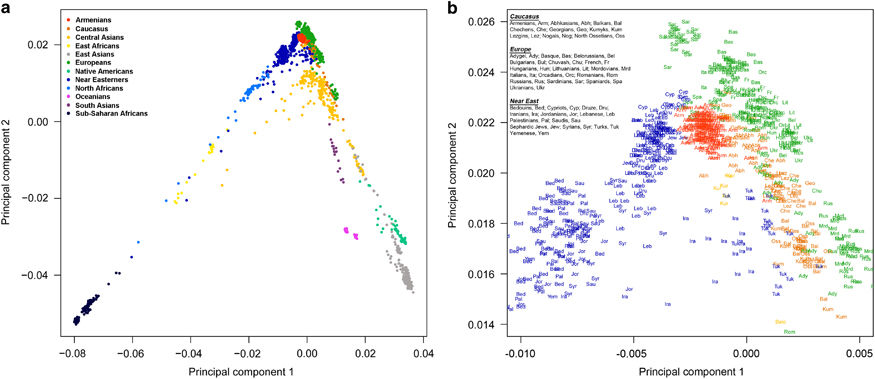
\includegraphics[width=\textwidth]{img/l04-genetics.jpg}
\end{center}

\begin{question}{}
What is $X$ for the genetic ancestry problem? What are the principal components? How were the principal components used to produce the figure above?
\end{question}

\subsection{Topic Modeling}

PCA also has many uses in natural language processing. It forms the basis for latent semantic indexing (see Deerwester 1990) and can also be used for topic modeling, a form of mixture model (see Section~\ref{sect:mixturemodels})\footnote{Figure: Topic modeling French crime fiction. From https://dragonfly.hypotheses.org/530.}.

\begin{center}
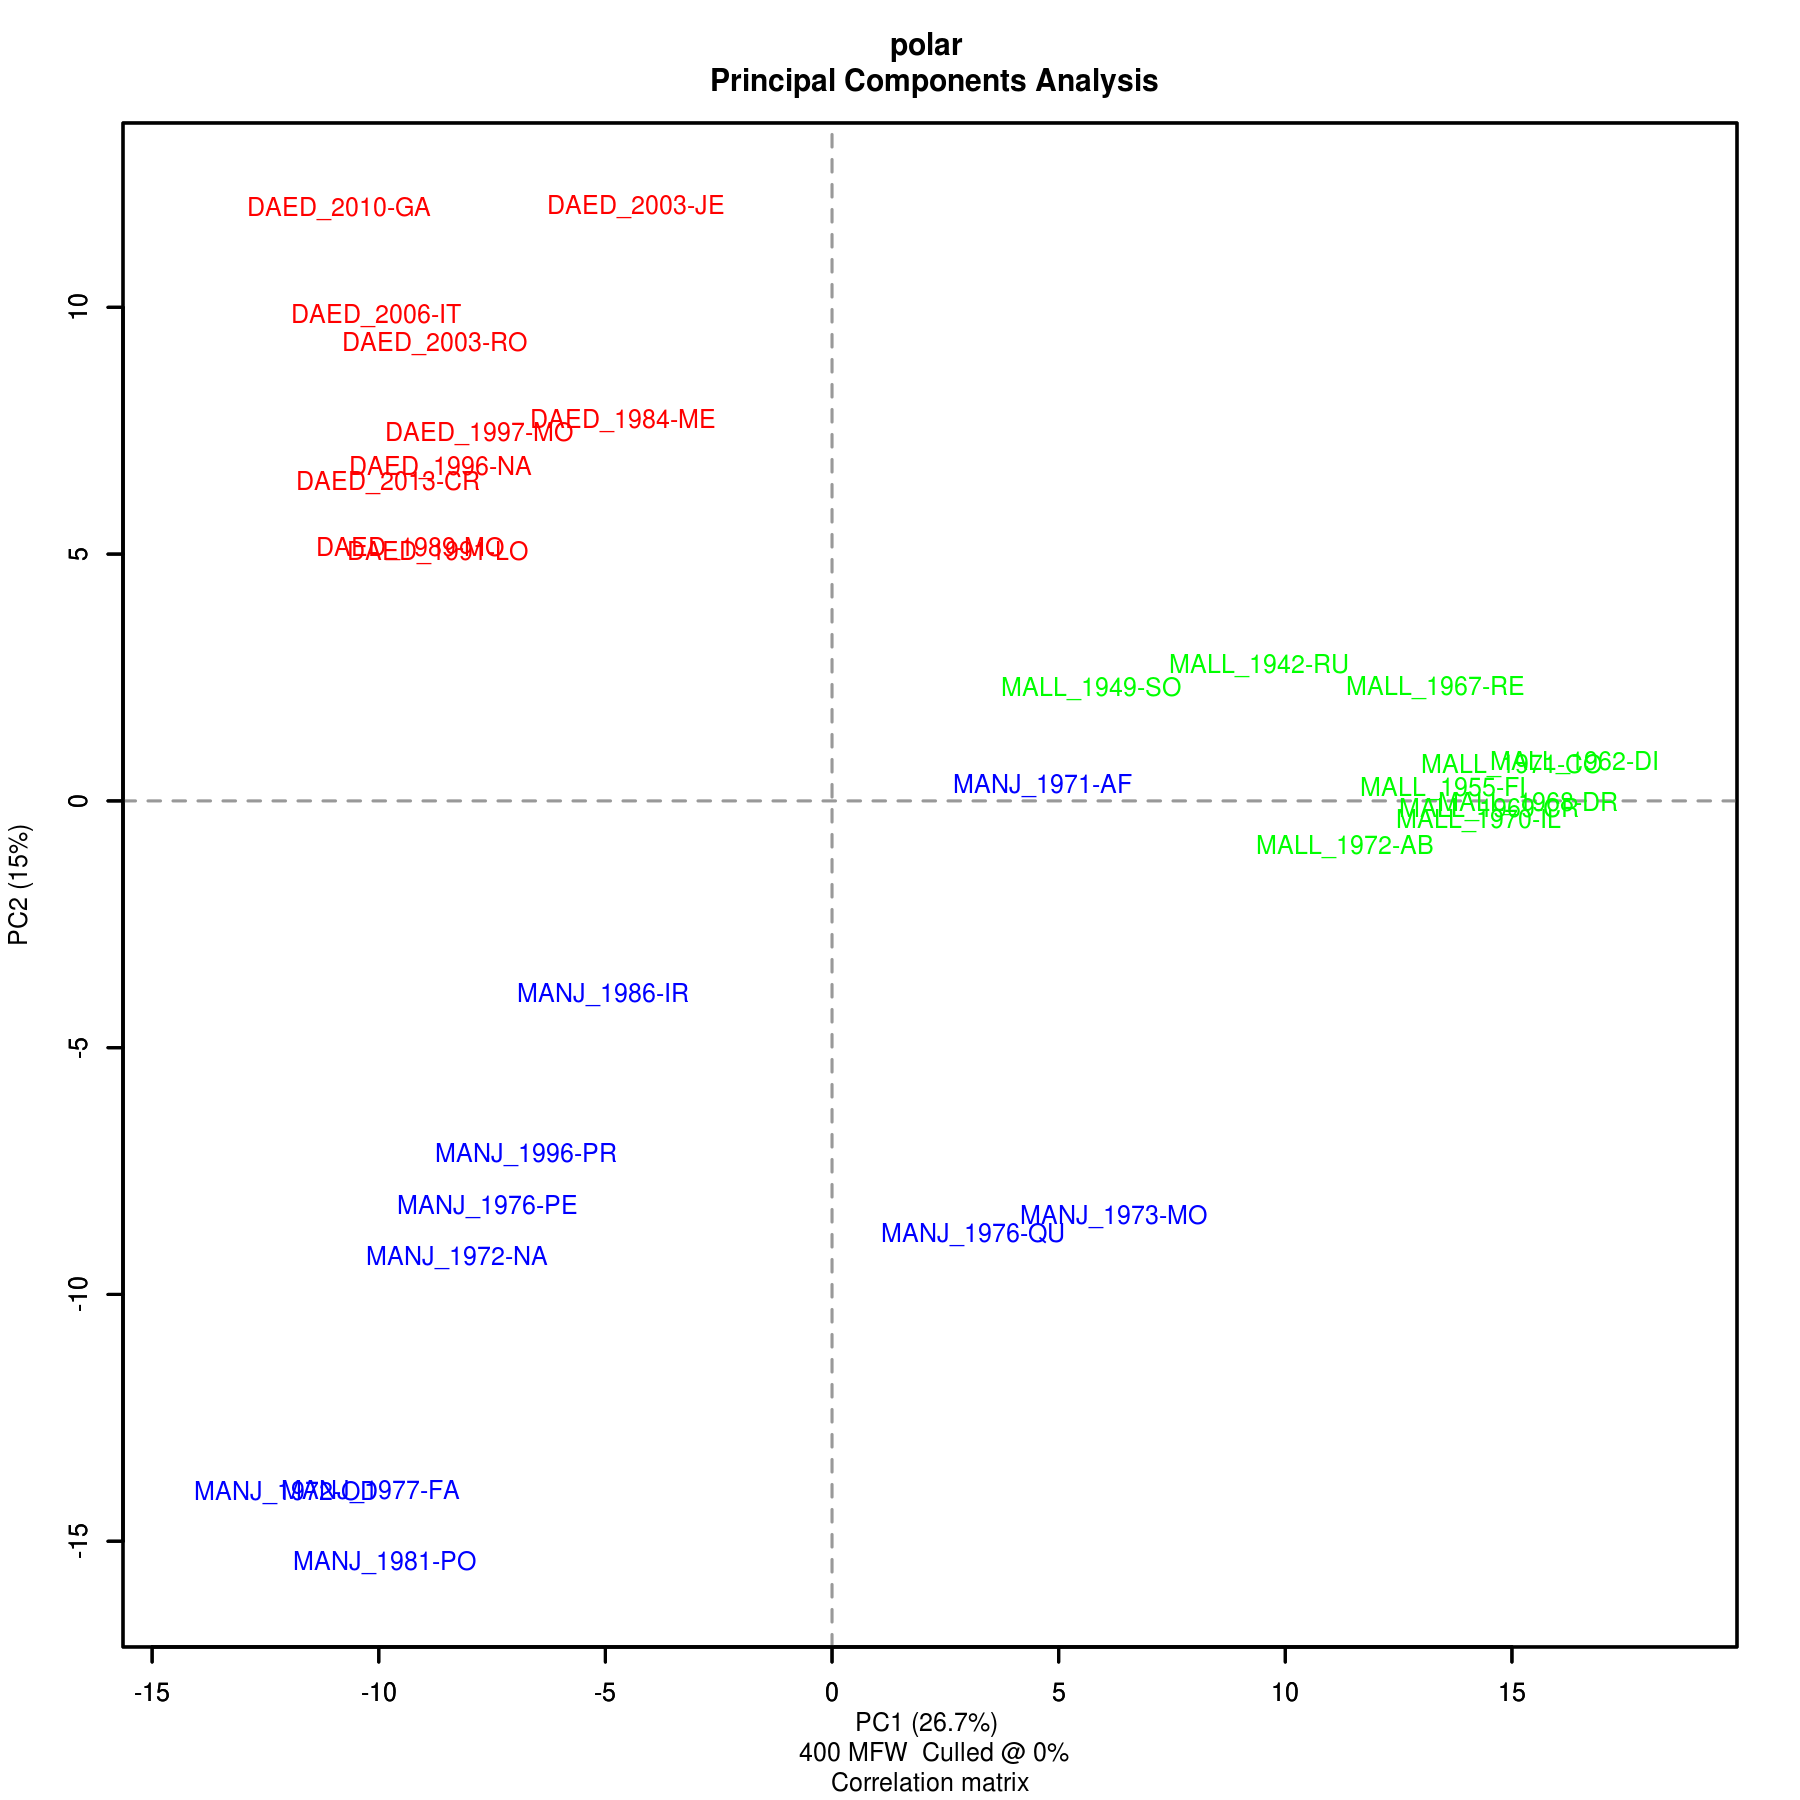
\includegraphics[width=0.7\textwidth]{img/l04-topics.png}
\end{center}

\begin{question}{}
What is $X$ for the topic modeling problem? For the latent semantic indexing problem? What do the principal components represent?
\end{question}

\begin{question}{}
Think of 2-3 different unsupervised learning problems from biology or medicine where PCA makes sense, conceptually at least, for modeling the data. How would you set up the data matrix in each case? What would the principal components correspond to in the data? 
\end{question}

%%%%%%%%%%%%%%%%%%%%%%%%%%%%%%%%%%%%%%%%%%%%%%%%%%%%%%%%%%%%%%%%%%%%%%%%%%%%%

\section{Technical Details (Advanced)}

\subsection{Eigenvalues and Eigenvectors \label{ssect:eig}}

One interpretation of matrix multiplication, $Ax$, where $A$ is an $m \times m$ square matrix and $x$ a vector of length $m$, is that $A$ linearly transforms $x$ by rotating it, changing its magnitude, or both. An \textbf{eigenvector} of $A$ is a vector that, when multiplied by $A$, grows or shrinks in magnitude but does not rotate. The multiplier of its magnitude is given by the corresponding \textbf{eigenvalue}. There are $m$ different eigenvalues and eigenvectors for an $m \times m$ matrix, although the eigenvalues may not all be distinct. The set of all eigenvalues of $A$ is called the \textbf{spectrum} of $A$. 

For all eigenvalue-eigenvector pairs, the relationship $Av = \lambda v$, where $v$ is an eigenvector and $\lambda$ its corresponding eigenvalue, must hold. To find the $\lambda$s and $v$s analytically, we can set the determinant $ | A - \lambda I | $, called the \textbf{characteristic polynomial}, equal to zero and solve for the eigenvalue and eigenvector corresponding to each root. Note that any scalar multiple of an eigenvector is itself an eigenvector; usually we restrict eigenvectors to have magnitude $1$ for this reason.

If a matrix is \textbf{symmetric} and \textbf{positive semidefinite} (all positive or zero eigenvalues), all of its eigenvectors will be orthogonal.

\subsection{PCA: Eigendecomposition Version} 

The first way we can find the principal components is by performing an eigen-decomposition identical to the one we performed in Section~\ref{ssect:eig} on the sample covariance matrix. The principal components will be the eigenvectors of this matrix, and the corresponding eigenvalues tell you how much of the dataset's overall variance is accounted for by each eigenvector.

One useful fact about the covariance matrix is that, because it is a symmetric matrix, it can be diagonalized:
\begin{equation} S = \frac{1}{n-1} X^T X = V L V^T \label{eqn:eigendiag} \end{equation}
where $V$ is a matrix of the $p$ eigenvectors of $S$ (each column is an eigenvector) and $L$ is a diagonal matrix with the eigenvalues of $S$ along the diagonal. This fact will be important later.

\subsection{PCA: Singular Value Decomposition (SVD) Version}

Although the eigendecomposition of the covariance matrix is generally the way PCA is presented, in practice most software uses another matrix decomposition called the \textbf{singular value decomposition (SVD)}, even though it is slower to compute, because it's more numerically stable.

Here's why the two methods are equivalent. Any matrix, $M$, with real or complex values (we'll focus on real valued matrices here) has an SVD of the form\footnote{This is in contrast with the eigendecomposition, which works only on positive semidefinite matrices.}:
$$ M = U D V^T $$
where $U$ is an orthogonal matrix, meaning that $U^TU = I$, $D$ is diagonal and all of its nonzero elements are non-negative real numbers called \textbf{singular values}, and $V$ is also orthogonal. For a square matrix, the SVD can be viewed as ``breaking up'' the transformation described by a matrix into three separate transformations: a rotation/reflection, a scaling, and another rotation/reflection\footnote{Figure: Graphical representation of the SVD of a square matrix, $M$. Note that the illustrator here uses $\Sigma$ instead of $D$ for the middle, diagonal matrix. Attribution: By Georg-Johann (Own work), via Wikimedia Commons.}:

\begin{center}

\includegraphics[width=0.5\textwidth]{img/l04-svd.pdf}
\end{center}

\noindent If we perform the SVD on $X$, we obtain a decomposition
$$ X = U D V^T $$
where $D$ is a diagonal matrix with singular values $d_1, \dots, d_p$. Knowing this, we can rewrite our covariance matrix as
\begin{align*} S &= \frac{1}{n-1} X^T X \\
&= \frac{1}{n-1} (UDV^T)^T U D V^T \\
&= \frac{1}{n-1} V D U^T U D V^T \\
&= V \frac{D^2}{n-1} V^T. \end{align*}

Comparing this to the form from Equation~\ref{eqn:eigendiag}, we see that the eigenvectors correspond to the right singular values of the SVD, and the eigenvalues are related to the singular values on the diagonal of $D$ by $\lambda_i = d_i^2/(n-1)$.

There are a lot of interpretations of the SVD. The one I like best is that the SVD provides a ``nearest orthogonal matrix'' to the original matrix. It's like the data have a coordinate system of orthogonal axes in which they most like to live, and the SVD tells you what that system is.

